Because the polar night jet is strongest in the late winter to early spring, we will consider the August-September-October (ASO) mean in our analysis of the PNJ. Sudden stratospheric warming events will also be discussed in this section. 

\subsubsection{Polar Night Jet}
As was discussed above, in all scenarios the PNJ shifts equatorward, in Control because the latitude of the highest temperature gradient shifts, in SAI 2020 and SAI 2080 because the temperature gradient in the lower stratosphere strongly increases. Figure \ref{fig:PNJ_UT_U_zmdiff} shows the zonal component of the integrated thermal wind and the anomalies in Control, SAI 2020 and SAI 2080 in ASO. As in section \ref{lowerstrat}, the observed wind and the integrated thermal wind show the same patterns, with the integrated thermal wind consistently higher than the observed wind due to friction effects. 

In Figure \ref{fig:PNJ_UT_U_zmdiff} we see that the PNJ indeed shifts equatorward in Control, confirming that the changes in the PNJ are governed by thermal changes under global warming. Its strength does not significantly changes either way. In SAI 2020 and SAI 2080 the PNJ shifts equatorward as well, also governed by thermal changes from SAI, but in contrast to Control the wind speed increases significantly. The pattern in SAI 2080 is the same as in SAI 2020, but the increase is at least 4 m/s less.

\begin{figure}[H]
	\centering
	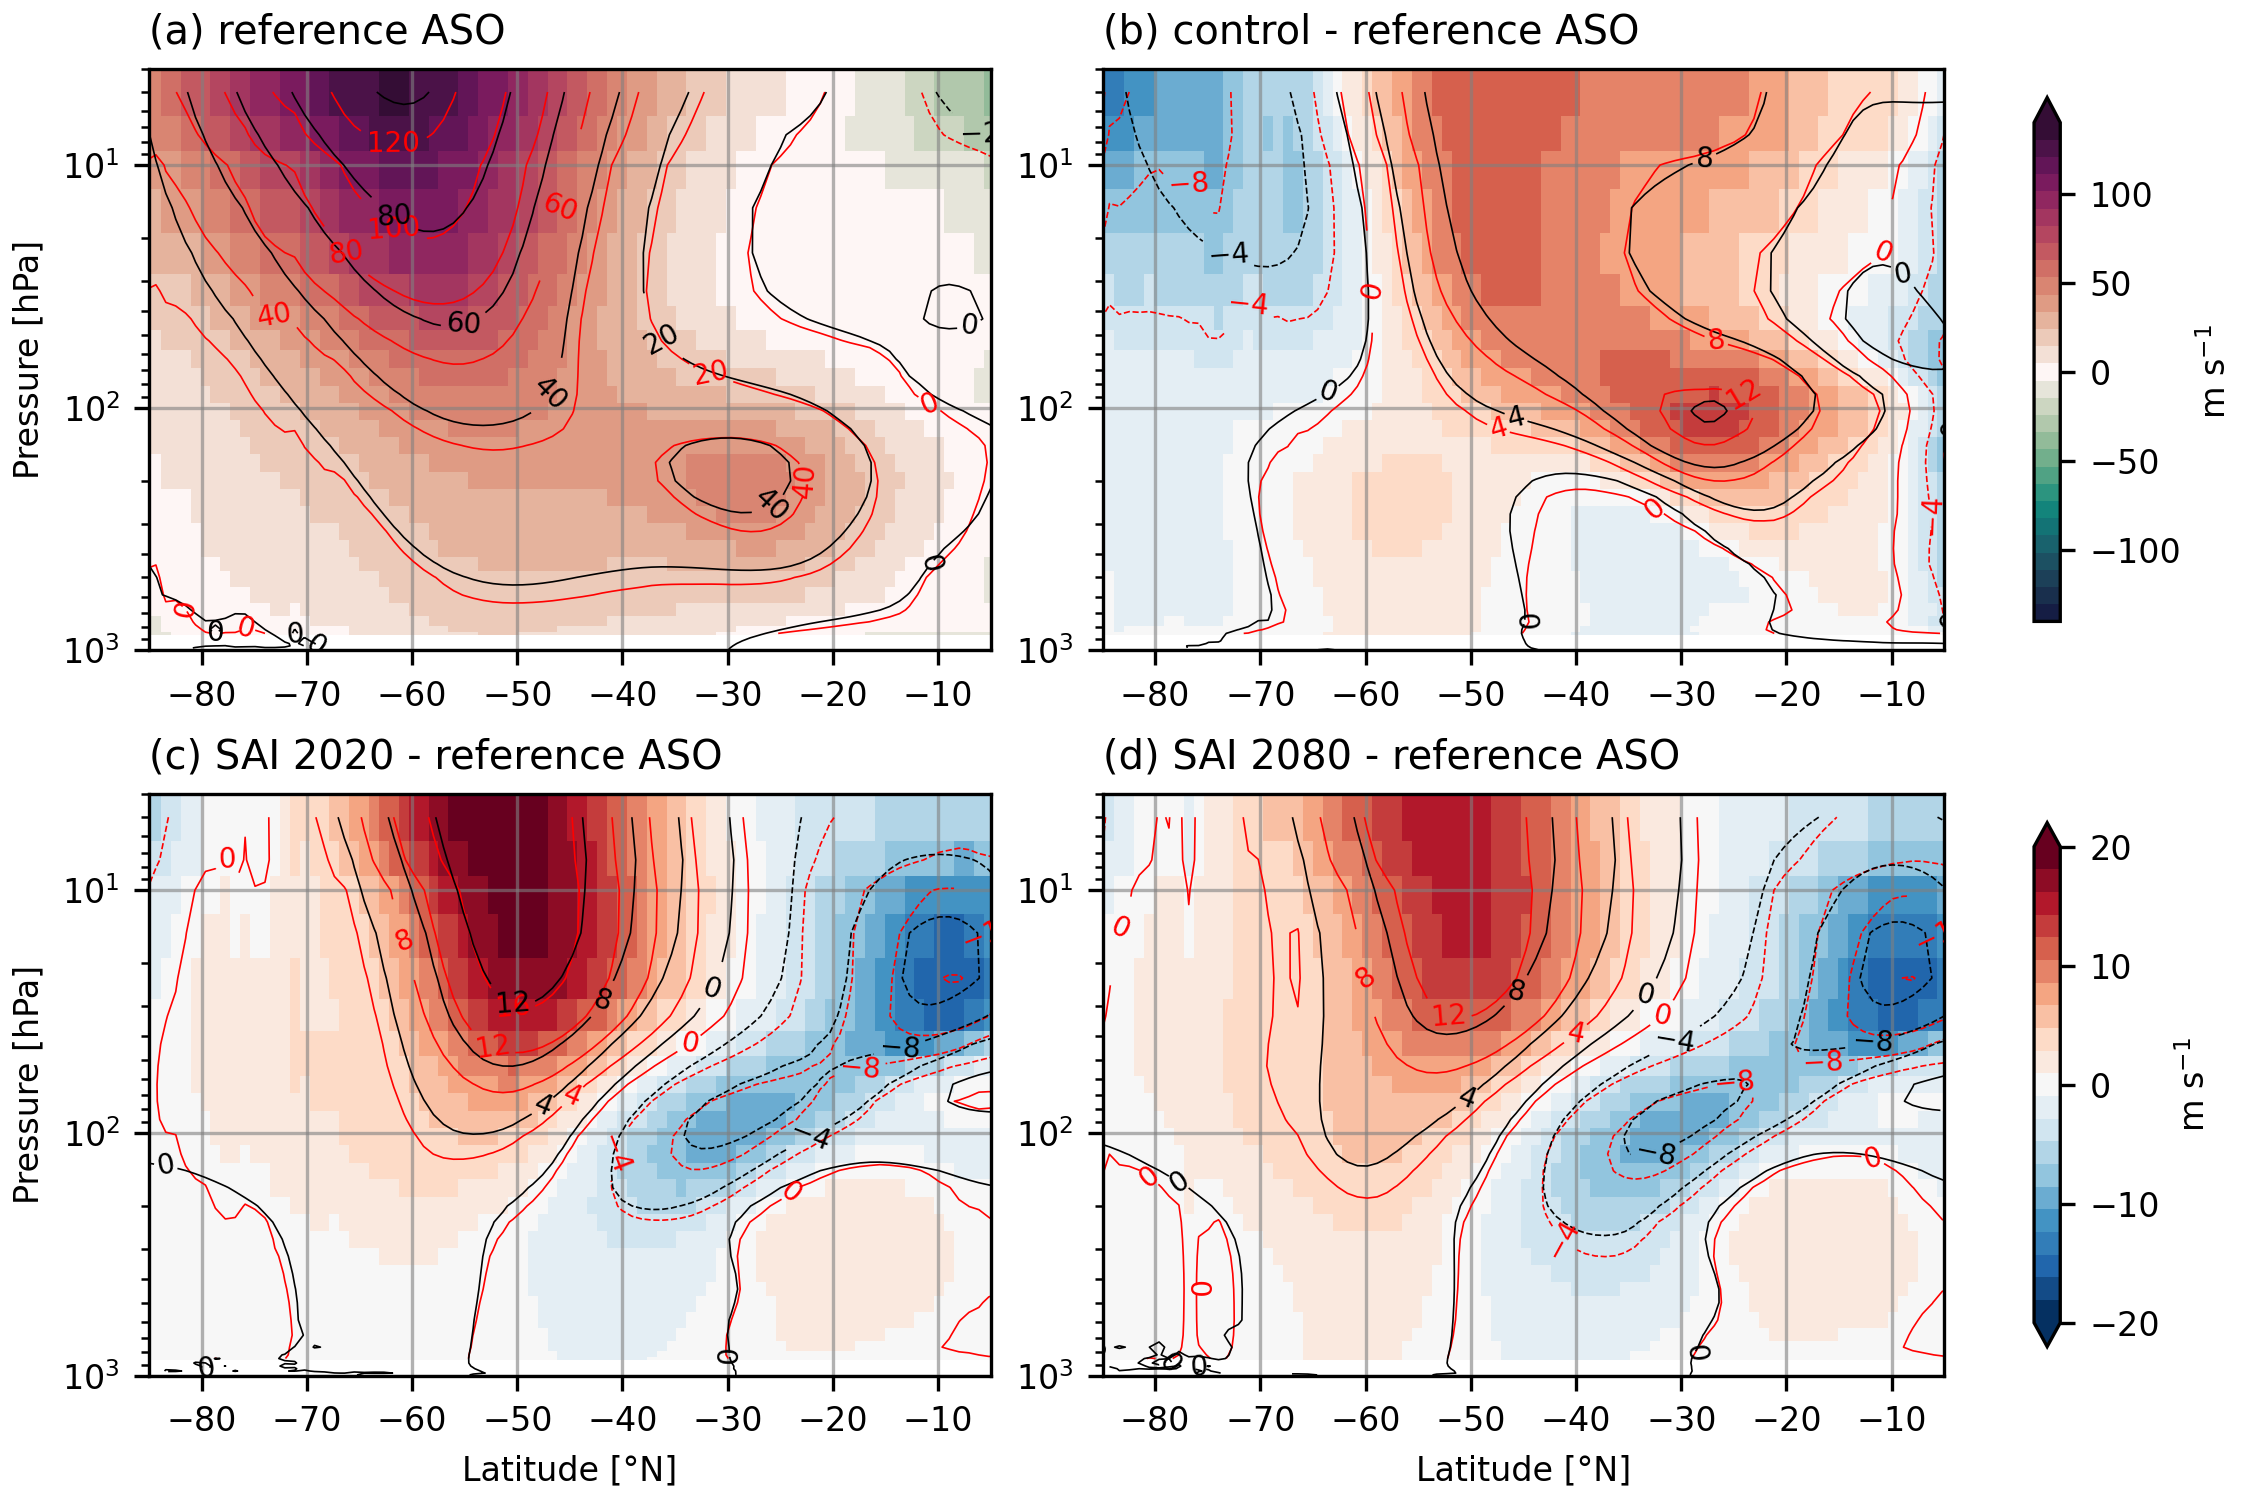
\includegraphics[width=0.95\linewidth]{images/PNJ_UT_U_zmdiff.png}
	\caption{ASO mean zonal-mean integrated thermal wind (shading and red contours) and zonal wind (contours, m/s) for (a): Reference; (b-d): Control, SAI 2020 and SAI 2080 anomaly compared to Reference.}
	\label{fig:PNJ_UT_U_zmdiff}
\end{figure}

The changes in kinetic energy per unit mass shown in Figure \ref{fig:PNJ_KE_U_zmdiff} correspond well with the changes in integrated thermal wind in Figure \ref{fig:PNJ_UT_U_zmdiff}. The eddy kinetic energy in Figure \ref{fig:PNJ_EKE_U_zmdiff} shows a different picture. In Control there is a stark decrease in EKE on the poleward side of the PNJ. This decrease is very large relative to the KE decrease, indicating a deacrease in eddy activity.

The decrease in EKE over the Antarctic is visible in SAI 2020 and SAI 2080 as well, though not as intensely. It still indicates a decrease in eddy activity. In the interior of the PNJ, where the KE increase is largest, the EKE shows a more broad increase. Most strikingly, in both SAI scenarios the EKE increases a little bit less where the zonal wind is strongest. Instead, the EKE increases the most on the flanks of the jet, indicating the jet becomes more broad and wavy. The magnitude by which this happens seems to correspond to the wind speed, as again SAI 2080 is slightly weaker than SAI 2020.


\begin{figure}[H]
	\centering
	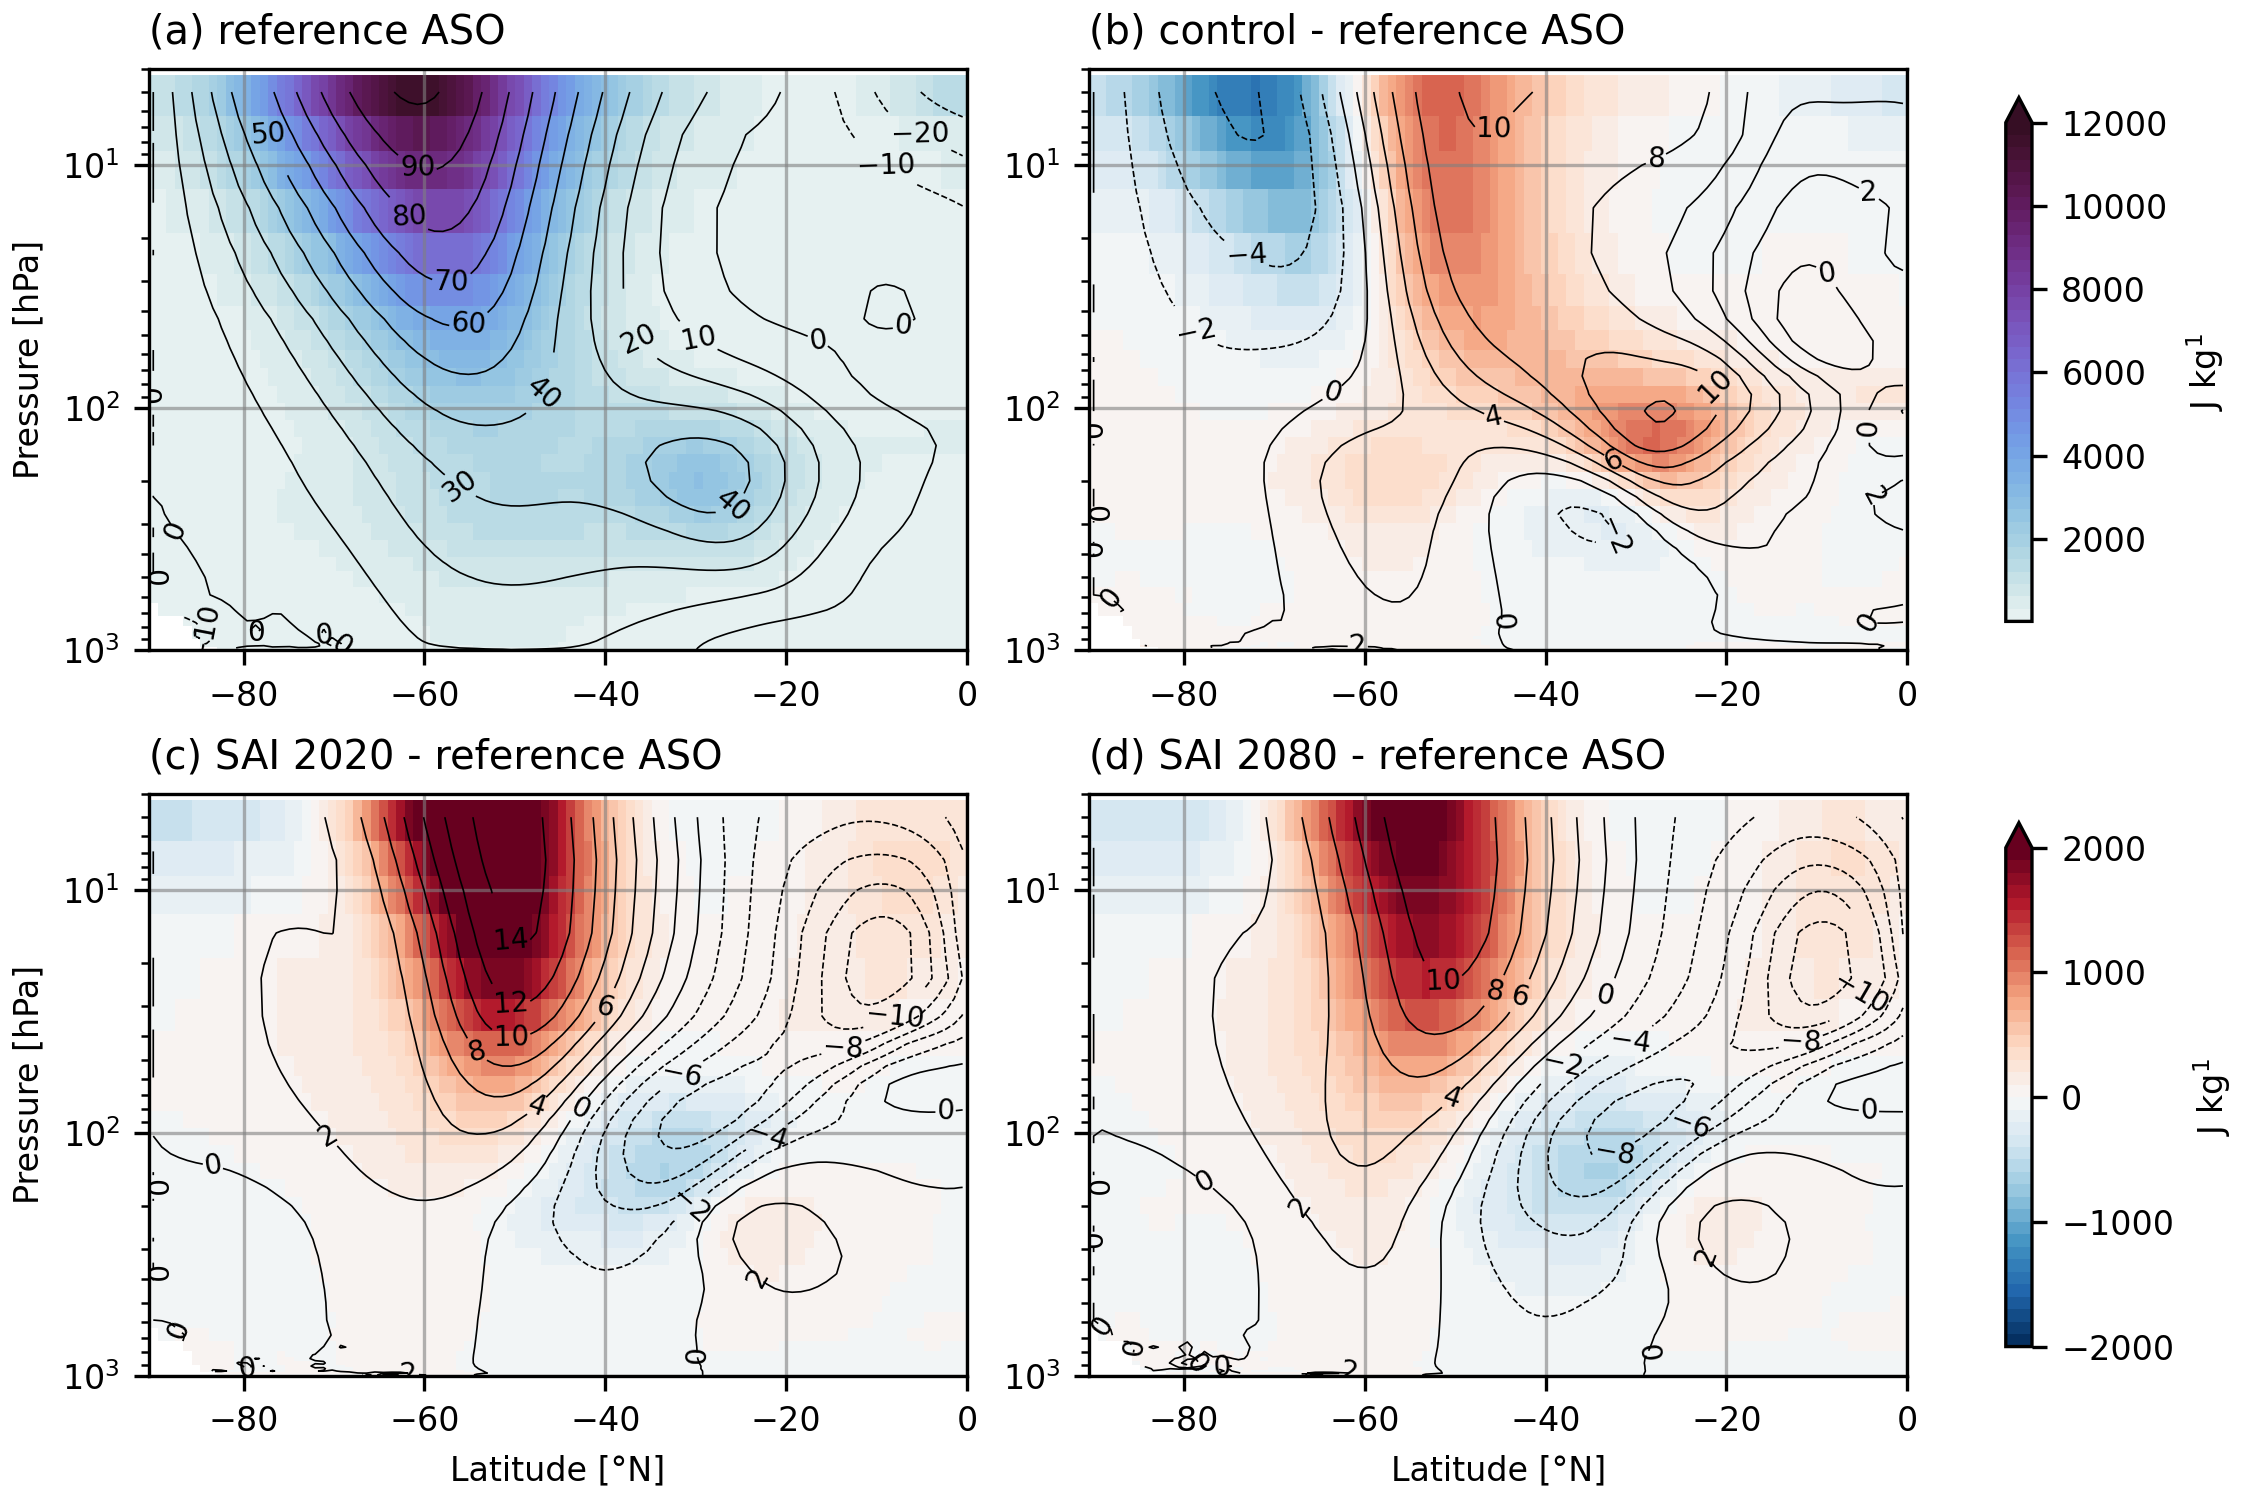
\includegraphics[width=0.95\linewidth]{images/PNJ_KE_U_zmdiff.png}
	\caption{JJA mean zonal-mean kinetic energy (shading) and zonal wind (contours, m/s) for (a): Reference; (b-d): Control, SAI 2020 and SAI 2080 anomaly compared to Reference.}
	\label{fig:PNJ_KE_U_zmdiff}
\end{figure}


\begin{figure}[H]
	\centering
	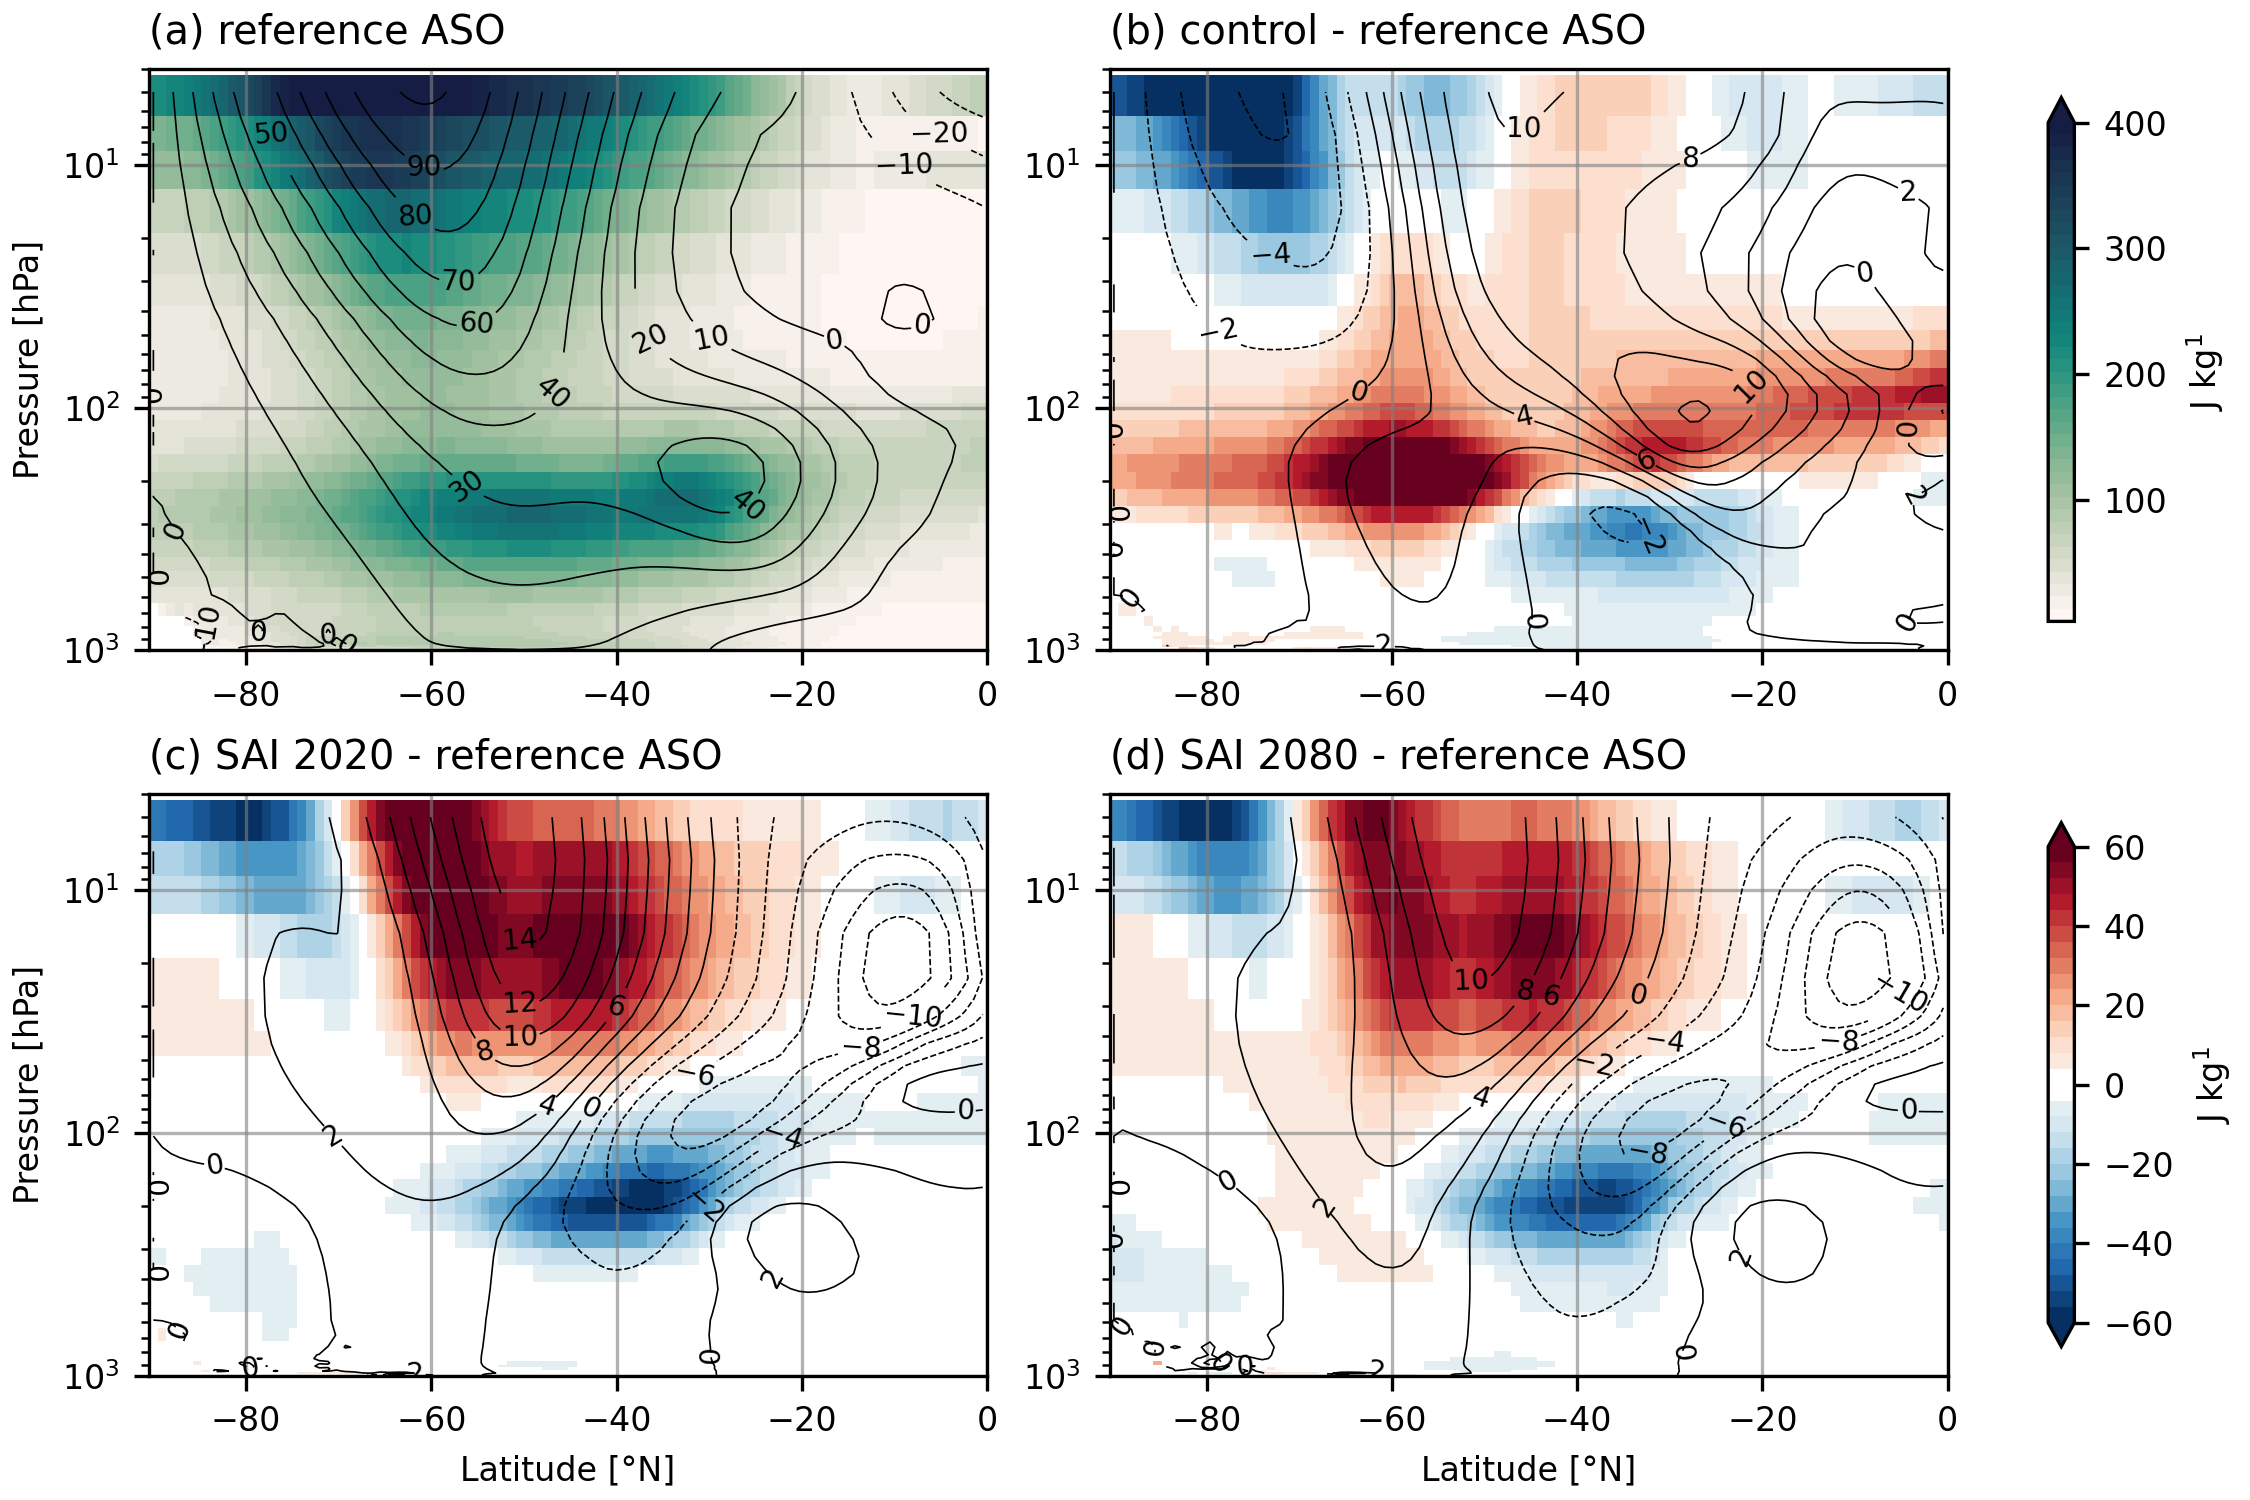
\includegraphics[width=0.95\linewidth]{images/PNJ_EKE_U_zmdiff.png}
	\caption{JJA mean zonal-mean eddy kinetic energy (shading) and zonal wind (contours, m/s) for (a): Reference; (b-d): Control, SAI 2020 and SAI 2080 anomaly compared to Reference.}
	\label{fig:PNJ_EKE_U_zmdiff}
\end{figure}

The intensity map of the PNJ is shown in Figure \ref{fig:PNJ_map}. The PNJ intensifies in all scenarios, most strongly in SAI 2020, followed by SAI 2080 and lastly Control. This increase in control was not apparend from the zonal mean figures, possibly because the increase is not zonally uniform. The PNJ indeed grows more broad in SAI 2020 and SAI 2080, as observed above. The equatorward shift in all scenarios is more clearly observed in Figure \ref{fig:PNJ_maxloc}, where the mean location of the maximum observed wind speed is shown. The scenario with the largest shift varies per location, with hardly any shift in any scenario in the 0°-60°E section, Control shifting the most in the 120°-180°E section, and SAI 2020 shifting the most in the 240°-300°E section. The shift in SAI 2080 is mostly consistent with SAI 2020, but deviates in the 240°-300°E section, coinciding with Control there instead. Maximum wind speed remains at Reference levels in Control, but increases by 8.0 m/s, or 8.3\%, in SAI 2020 and 6.2 m/s, or 6.4\%, in SAI 2080.

\begin{figure}[H]
	\centering
	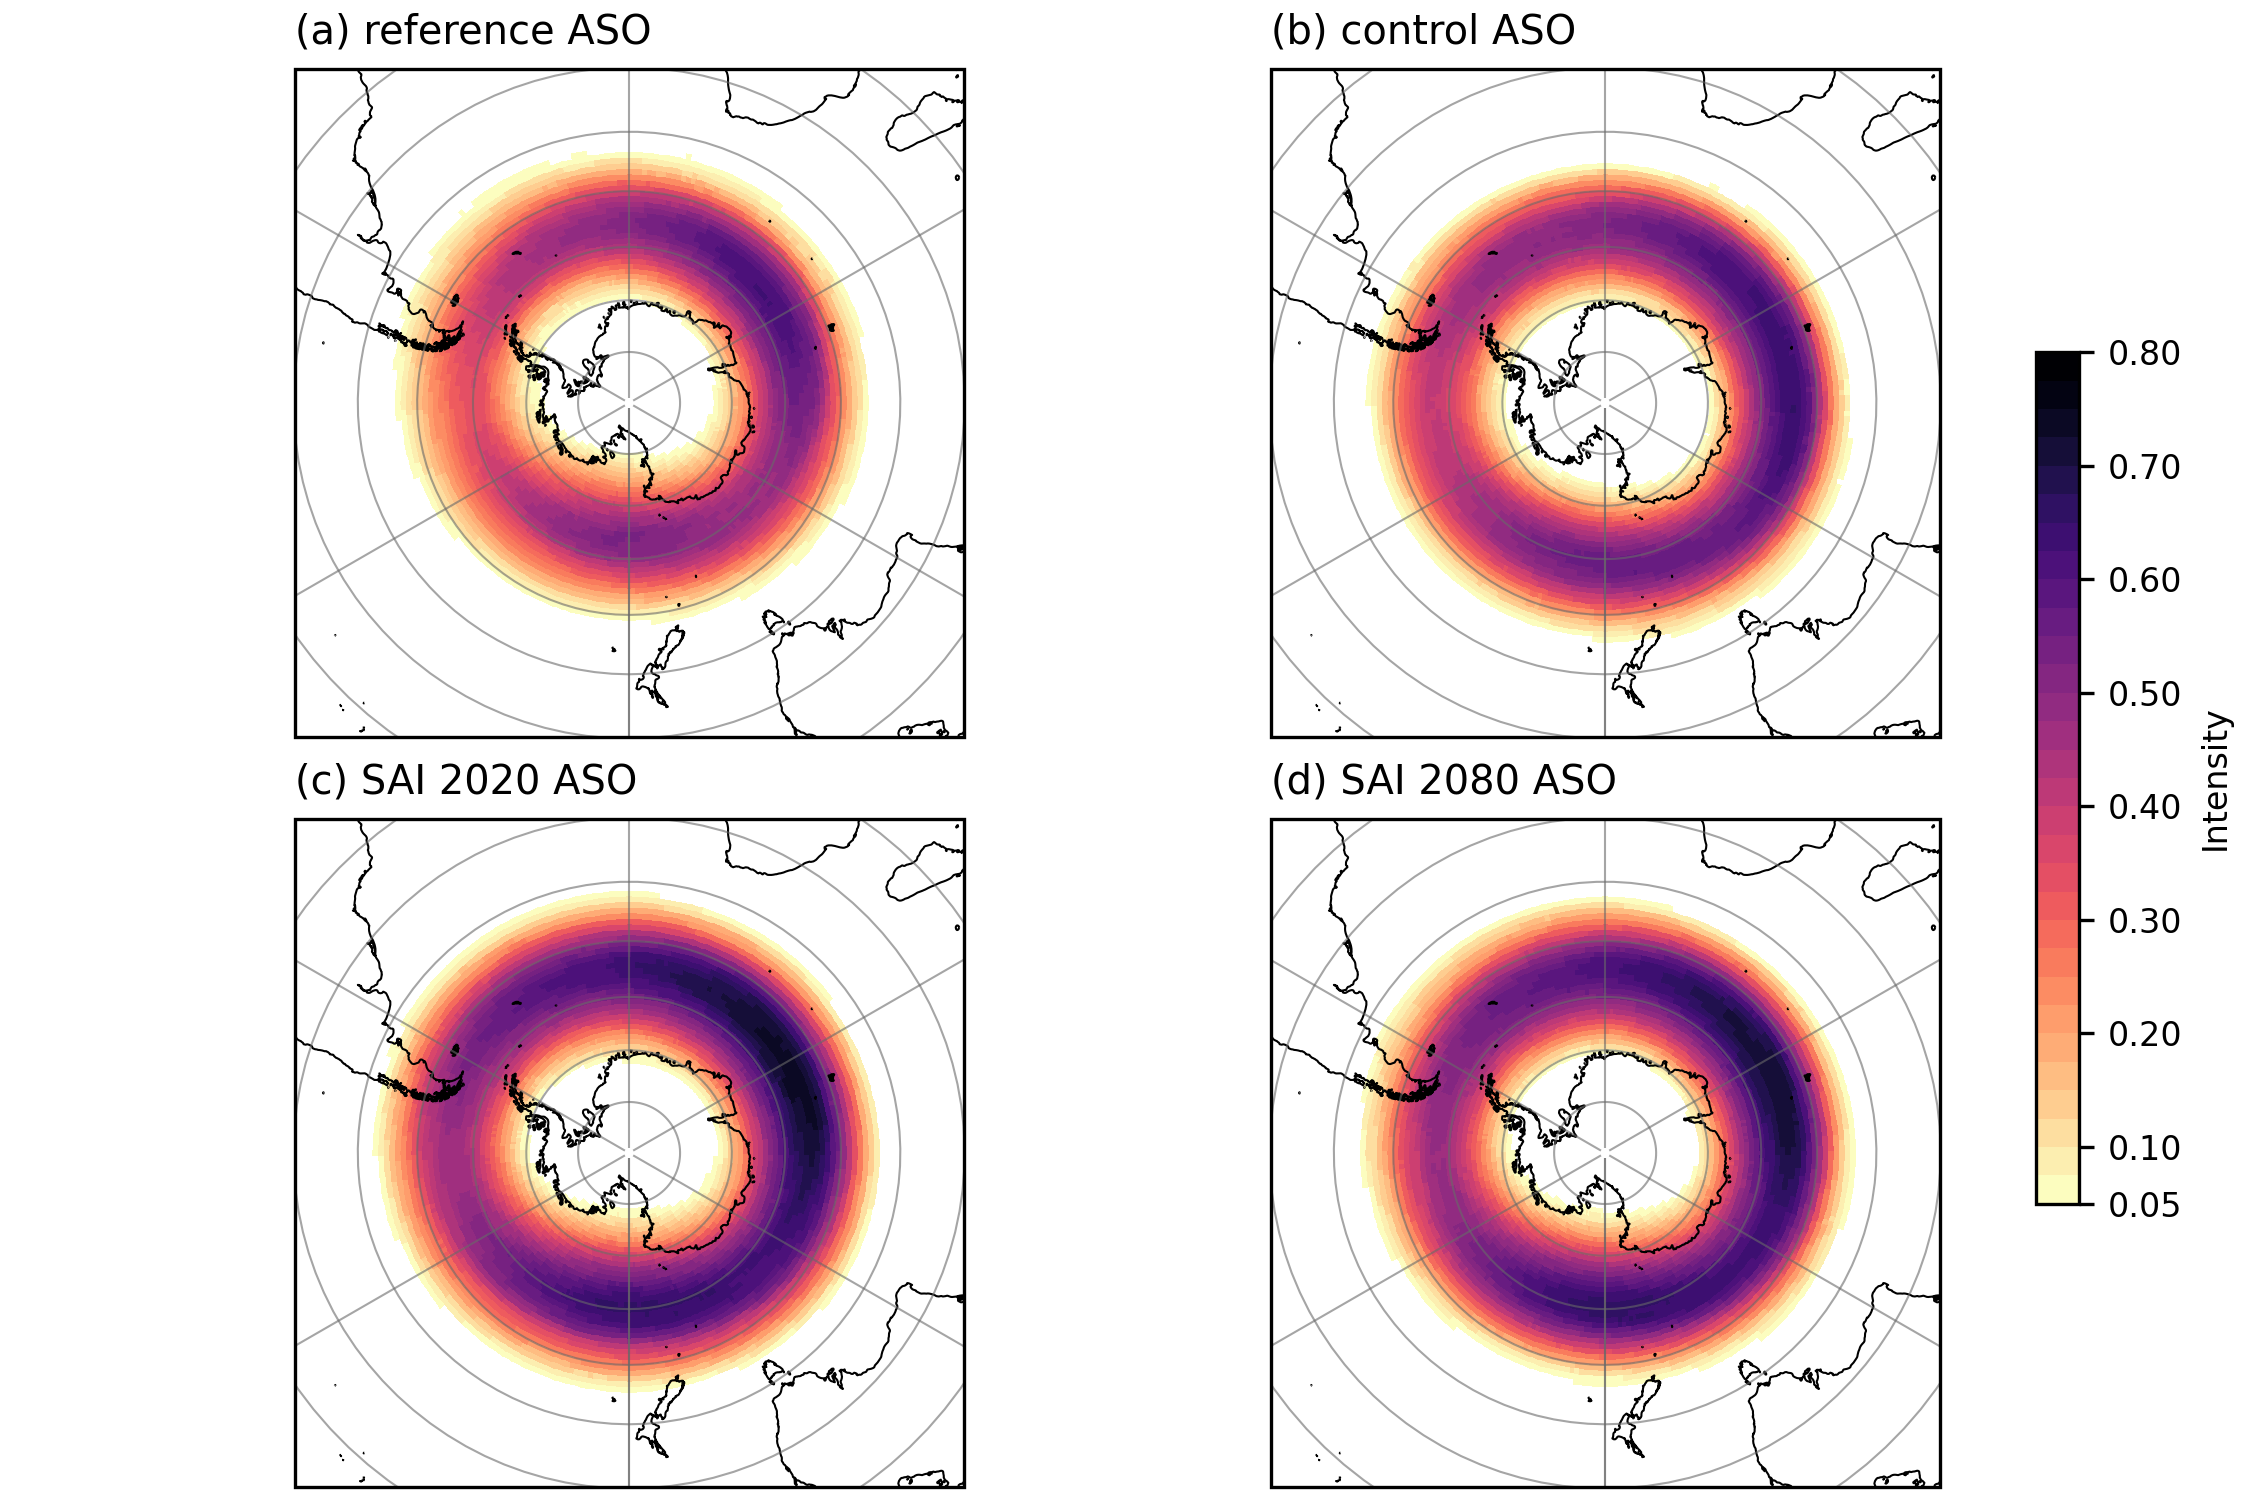
\includegraphics[width=0.95\linewidth]{images/PNJ_map.png}
	\caption{Polar night jet intensity map of zonal wind, values counted when the threshold of 80 m/s was passed at 10 hPa, for (a) Reference, (b) Control, (c) SAI 2020 and (d) SAI 2080. 0°E is oriented towards the top of the figure.}
	\label{fig:PNJ_map}
\end{figure}


\begin{figure}[H]
	\centering
	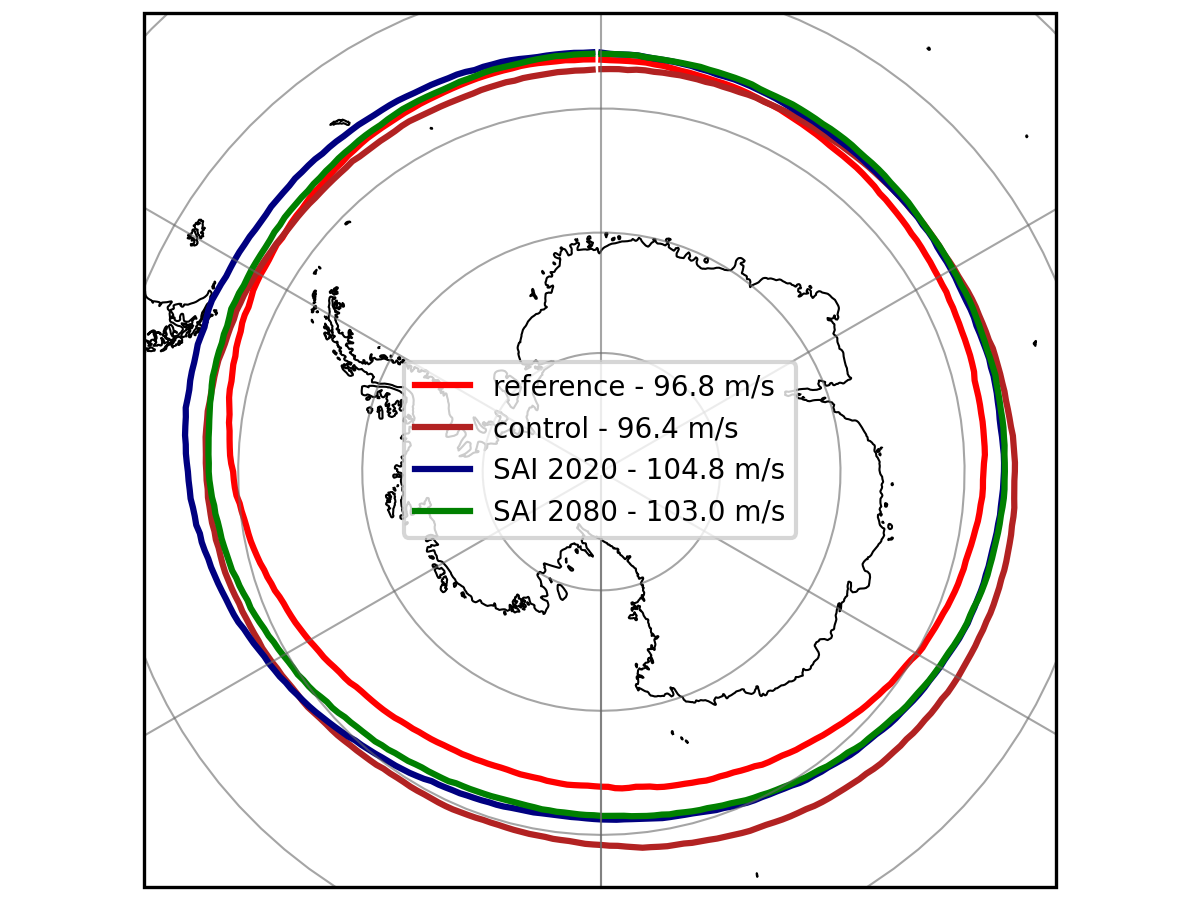
\includegraphics[width=0.48\linewidth]{images/PNJ_maxloc_latlon.png}
	\caption{Mean location of maximum wind speed at 10 hPa, with longitudinal mean maximum wind speed, for Reference, Control, SAI 2020 and SAI 2080. 0°E is oriented towards the top of the figure.}
	\label{fig:PNJ_maxloc}
\end{figure}

\subsubsection{Sudden Stratospheric Warming Events}
The decrease in EKE over the Antarctic observed in \ref{fig:PNJ_EKE_U_zmdiff} suggests a decrease in the occurence of sudden stratospheric warming events (SSW). Figure \ref{fig:PNJ_climographTU} shows the area weighted mean temperature of the 10 hPa level above 60°S, together with the zonal wind at 10 hPa and 60°S. In Reference there is a number of years where the temperature increases, and a number of years the zonal wind decreases compared to the mean. Though not explicitly identified, this happens in pairs, when the temperature rises, the winds decrease. In Control the frequency of these SSW-like conditions decreases significantly, the temperature and zonal wind bands narrow compared to Reference. In SAI 2020 there appears to be one year with SSW-like conditions, but again the temperature and zonal wind bands narrow. SAI 2080 shows the same trend. 

In all scenarios the zonal wind increases, as was already discussed in the results above, and the temperature decrease due to increased greenhouse gases is also visible. In all scenarios the PNJ forms earlier in the year, surpassing 80 m/s in early to mid-July in Control and in mid-June in SAI 2020 and SAI 2080, as opposed to mid-July in Reference. The PNJ also dissolves later in the year, decreasing to 80 m/s in late October in Control and early November in SAI 2020 and SAI 2080, as opposed to mid-October in Reference.

\begin{figure}[H]
	\centering
	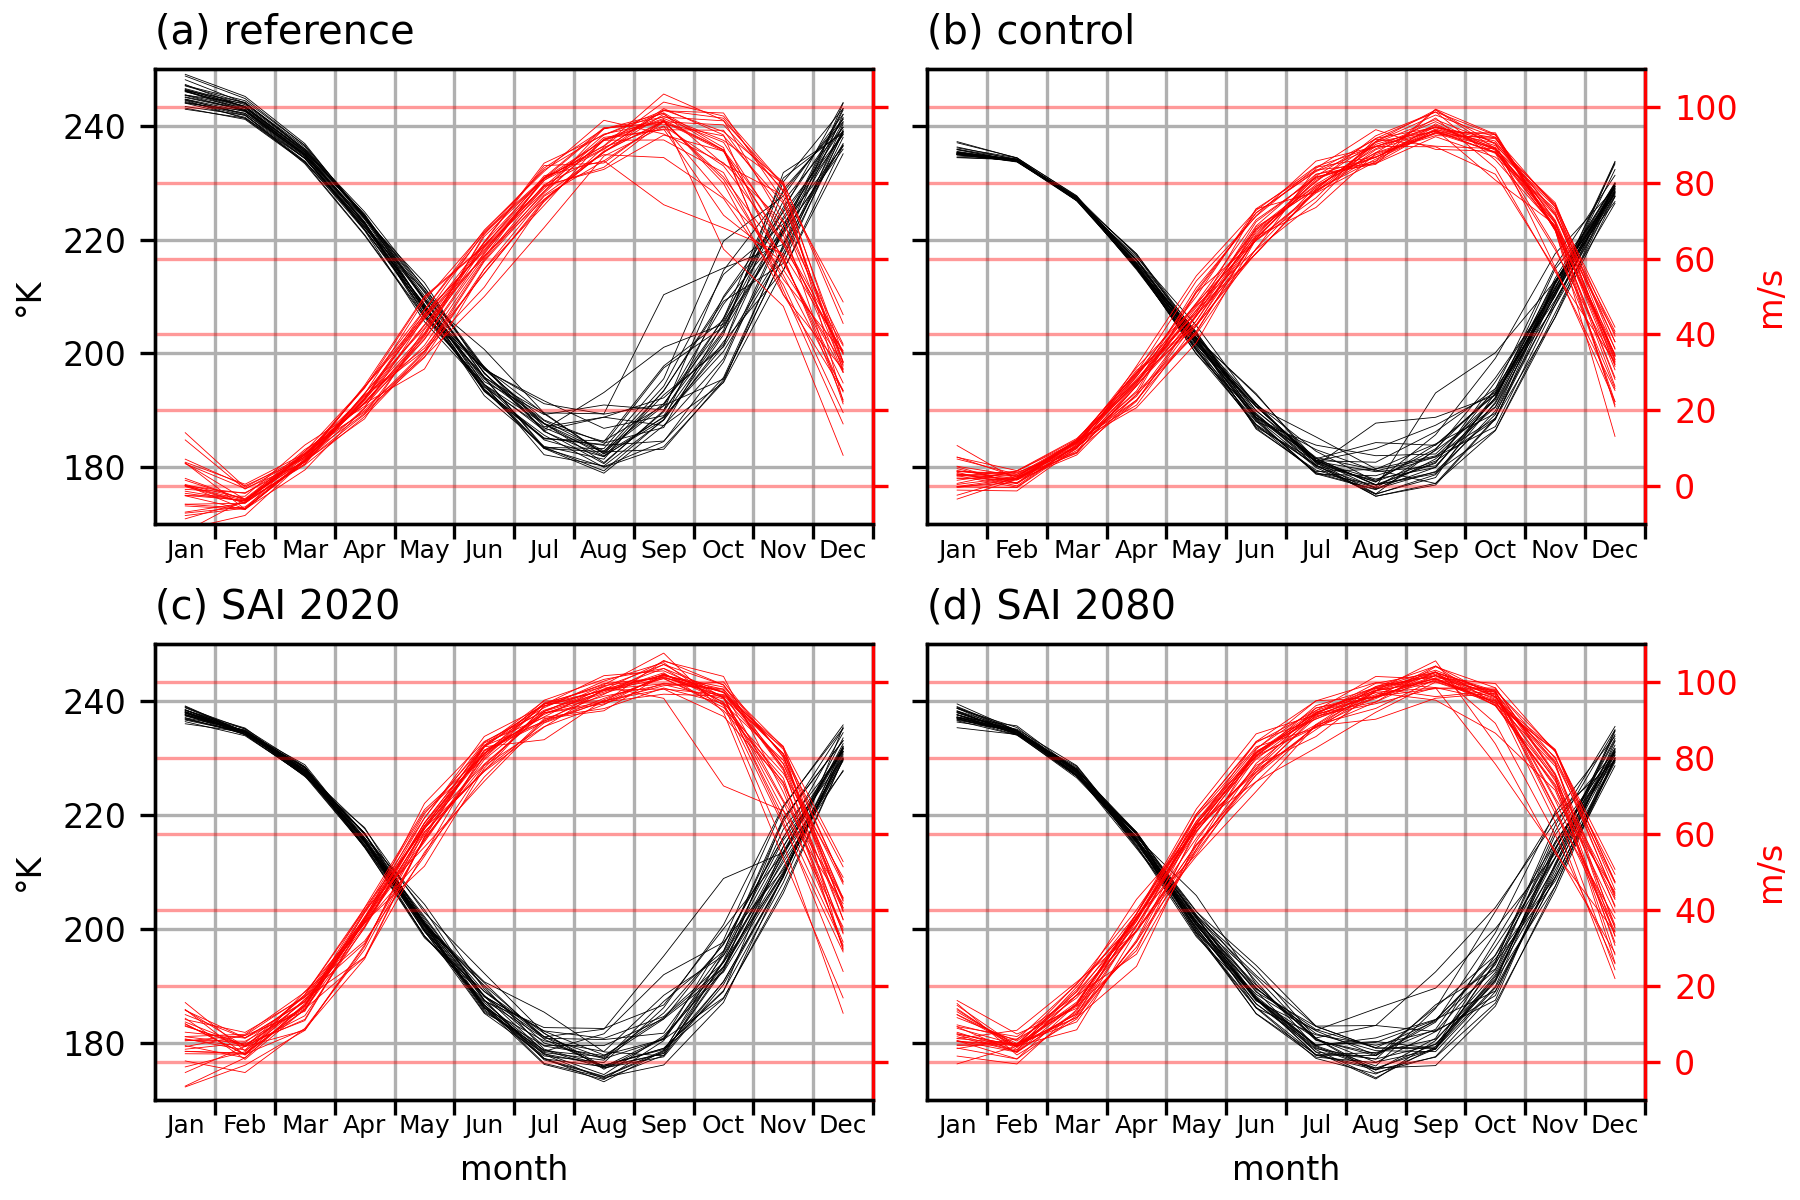
\includegraphics[width=0.95\linewidth]{images/PNJ_climographTU.png}
	\caption{Climograph of area-weighted mean temperature of 60°-90°S at 10 hPa (black) and zonal-mean zonal wind at 60°S and 10 hPa (red) for (a) 2016-2045 and (b) 2101-2130 in the SSP5-8.5 experiment, (c) 2101-2130 in the gradual SAI experiment and (d) 2101-2130 in the rapid cooling SAI experiment.}
	\label{fig:PNJ_climographTU}
\end{figure}